\documentclass[main.tex]{subfiles}
\pagestyle{main}

\begin{document}
\chapter{Structuration des codes de calculs \label{chap:structure_code} }
\mylettrine{D}{e} nombreux codes de calculs ont été développés durant la thèse. Outre le début de la thèse qui s'est déroulée sous Scilab dans le but de maquetter rapidement le code résolvant les différents modèles EDP, plusieurs codes ont été élaborés dans différents langages. 
Sans tomber dans la présentation détaillée de l'ensemble des codes de calcul,  %développés pendant ma thèse, 
faisons en un tour d'horizon. 
Ma thèse étant divisée en deux grandes parties, deux codes ont été 
implémentés~: 
%% développés~:
\begin{myitemize}
\item le premier, pour résoudre le modèle EDP et fournir des simulations numériques qui reproduisent des croissances tumorales et des résistances aux traitements,
\item le second, pour calculer un quantificateur de l'\hetero à partir d'une image, que ce soit une image provenant directement de l'appareil d'imagerie médicale ou une image provenant de la simulation numérique.
\end{myitemize}  

\section{Code de calcul pour la simulation numérique du modèle EDP\label{sec:code_modeleEDP}}
Le code permettant la simulation numérique via le modèle EDP a été développé en C++, avec la librairie eLYSe. Cette librairie, commune à toute l'équipe de recherche et développée par Olivier Saut, est une interface qui fournit un certain nombre de solveurs pour les problèmes classiques (transport et diffusion) traités par une méthode de volumes finis sur maillages cartésiens. Elle est multi-plateforme (Linux et MacOS). 
Elle s'appuie sur la librairie d'algèbre linéaire PETSc~\cite{balay2014petsc,balay2012petsc}, bien qu'aucune connaissance de PETSc ne soit nécessaire pour utiliser eLYSe. 
Ceci est principalement du au fait de la présence des structures de types Field (tableaux 2D et 3D) que cette librairie fournit. 

\paragraph{}
Après avoir appris le C++, j'ai pu prendre en main cet outil. Divers modules ont pu être construits~:
\begin{myitemize}
\item Un module pour les schémas à stencil croisé (de type \twinweno)
\item Un module fournissant diverses géométries en fonction de paramètres permettant de construire la condition initiale du modèle EDP.
\item Une classe Modele qui est à même de calculer, en fonction de paramètres (ceux fournis dans le chapitre~\ref{chap:modele_EDP}, dans la Table~\ref{table_variable} de la  page~\pageref{table_variable}) l'évolution spatio-temporelle des différentes quantités du modèle EDP (notamment les diverses populations de cellules). 
Cette classe contient entre autres~:
\begin{myitemize}[label=--]
\item la définition des paramètres et leurs affectations,
\item les allocations mémoire des variables intervenant dans le modèle EDP,
\item les schémas en temps et le calcul de CFL, 
\item les interactions entre les populations et la vascularisation, 
\item les points de contrôle (les populations sont-elles toujours comprises entre 0 et 1, moyennant une certaine tolérance ?),
\item les sorties fichiers.
\end{myitemize}
\item Une classe de méta-modèle, permettant d'explorer, de différentes manières, l'espace des paramètres lié à un modèle. Cette classe m'a notamment servie pour réaliser le fit (présenté sur la Figure~\ref{fig:fit_area_henbert}, page~\pageref{fig:fit_area_henbert}, dont les paramètres sont présentés dans la Table~\ref{table_param} page~\pageref{table_param}) des données cliniques par le modèle EDP. Plusieurs méthodes d'exploration ont été abordées : Monte-Carlo~\cite{spall2005introduction}, méthode de sensitivité ou de descente, algorithmes génétiques~\cite{davis1987genetic,goldberg1994algorithmes}... 
\end{myitemize}

Le modèle EDP ayant beaucoup de paramètres et admettant beaucoup de minima locaux, il n'a pas été facile d'obtenir un fit acceptable du volume tumoral. Les fits présentés dans ce manuscrit représentent  donc des minima locaux de l'erreur $L^2$, et non des minima globaux. La méthode adoptée est la suivante~: 
\begin{myenumerate}
\item Méthode de Monte Carlo. Des méthodes où l'on choisit de mailler l'espace des paramètres ont également été examinées. Le nombre de paramètres étant importants cette méthode a finalement été écartée car beaucoup trop coûteuse. 
\item Après avoir réalisé des centaines de simulations avec des jeux de paramètres aléatoires, les meilleurs candidats ont été examinés de plus près. Pour chacun d'eux, une analyse de sensibilité a été effectué sur chaque paramètres afin de comprendre localement l'influence de ceux-ci sur le modèle.
\item Pour les meilleurs candidats, une méthode de descente, combinée à de nombreuses interventions manuelles, a finalement été effectuée pour converger vers un minimum de l'erreur $L^2$. 
\end{myenumerate}


Le code de calcul est séquentiel. La partie recherche d'optimum dans l'espace des paramètres a elle été (pseudo-)parallélisée. A un jeu de paramètres donné, il y a un modèle qui est calculé sur un seul et  unique processeur. Les méthodes d'exploration de l'espace des paramètres nécessitant l'évaluation de plusieurs modèles, on partage l'ensemble des évaluations à réaliser entre les différents processeurs. Par exemple, sur une méthode de gradient, à chaque pas de l'algorithme, une approximation du gradient (dérivée du modèle par rapport à ses $n$ paramètres ici) est requise. Ainsi pour chaque paramètre, une évaluation est nécessaire. Chaque évaluation est réalisée sur une seul et unique processeur, mais on partage les $n$ évaluations requises sur le nombre de processeurs disponibles.


Pour donner un ordre d'idée du code manipulé, présentons le en quelques chiffres. Ce code est subdivisé en une dizaine de modules conduisant à un total d'environ \numprint{10000} lignes. Il est exécuté sur la plateforme de calcul INRIA, nommée PlaFRIM, sans laquelle de nombreuses simulations numériques n'auraient pas pu être réalisées. Le temps moyen d'exécution d'une simulation est d'environ~1h30. 


\section{Code de calcul aboutissant à la quantification de l'\hetero}
Le code de calcul générant le pourcentage d'\hetero aussi bien clinique que numérique est très hétéroclite. Il y a plusieurs raisons à cela :
\begin{myitemize}
\item On veut pouvoir manipuler des données de natures différentes. On souhaite générer les histogrammes des niveaux de gris depuis des sources diverses :
\begin{myitemize}[label=$-$]
\item Les données cliniques sont dans un format particulier~: le format DICOM. C'est un format de méta-image, qui nécessite l'utilisation d'un logiciel (ou d'une librairie) spécifique pour être visualisé et traité. 
\item La simulation numérique fournit les différentes populations~$P,N$ et~$S$. A partir de cela et des niveaux de gris associés~$\tau_P, \tau_N$ et~$\tau_S$, une image scanner est synthétisée.
\end{myitemize}
\item Le code s'appuie sur des langages différents :
\begin{myitemize}[label=$-$]
\item C++, avec la librairie ITK. Passage quasiment obligatoire (il y a très peu d'alternative) pour pouvoir traiter des données au format DICOM.
\item Python, avec la librairie Scikit-learn~\cite{pedregosa2011scikit}, qui contient un module dédié au mélange gaussien.
\end{myitemize}
\end{myitemize}

Au niveau des données, il n'y a pas que la nature des images qui diffère~: le moyen d'acquérir le contour diffère également. 
Pour les données cliniques, grâce au logiciel OsiriX~\cite{rosset2004osirix,ratib2006open}, nous pouvons contourer manuellement les tumeurs, et en exporter le contour au format xml. 
En ce qui concerne les images provenant de la simulation numérique, il n'y a pas de contour défini. Le choix (assez naturel) a été fait de le définir en prenant un seuil sur la population saine. Moyennant un parseur\footnote{\correction{Analyseur syntaxique, qui permet de dissocier, dans un fichier écrit en un certain  langage (XML ici), le fond de la forme et de la structure propre au langage.}} XML, on peut donc se ramener à un contour semblable dans les deux cas.

\begin{sidewaysfigure}
%%\begin{figure}
\centering
\vfill
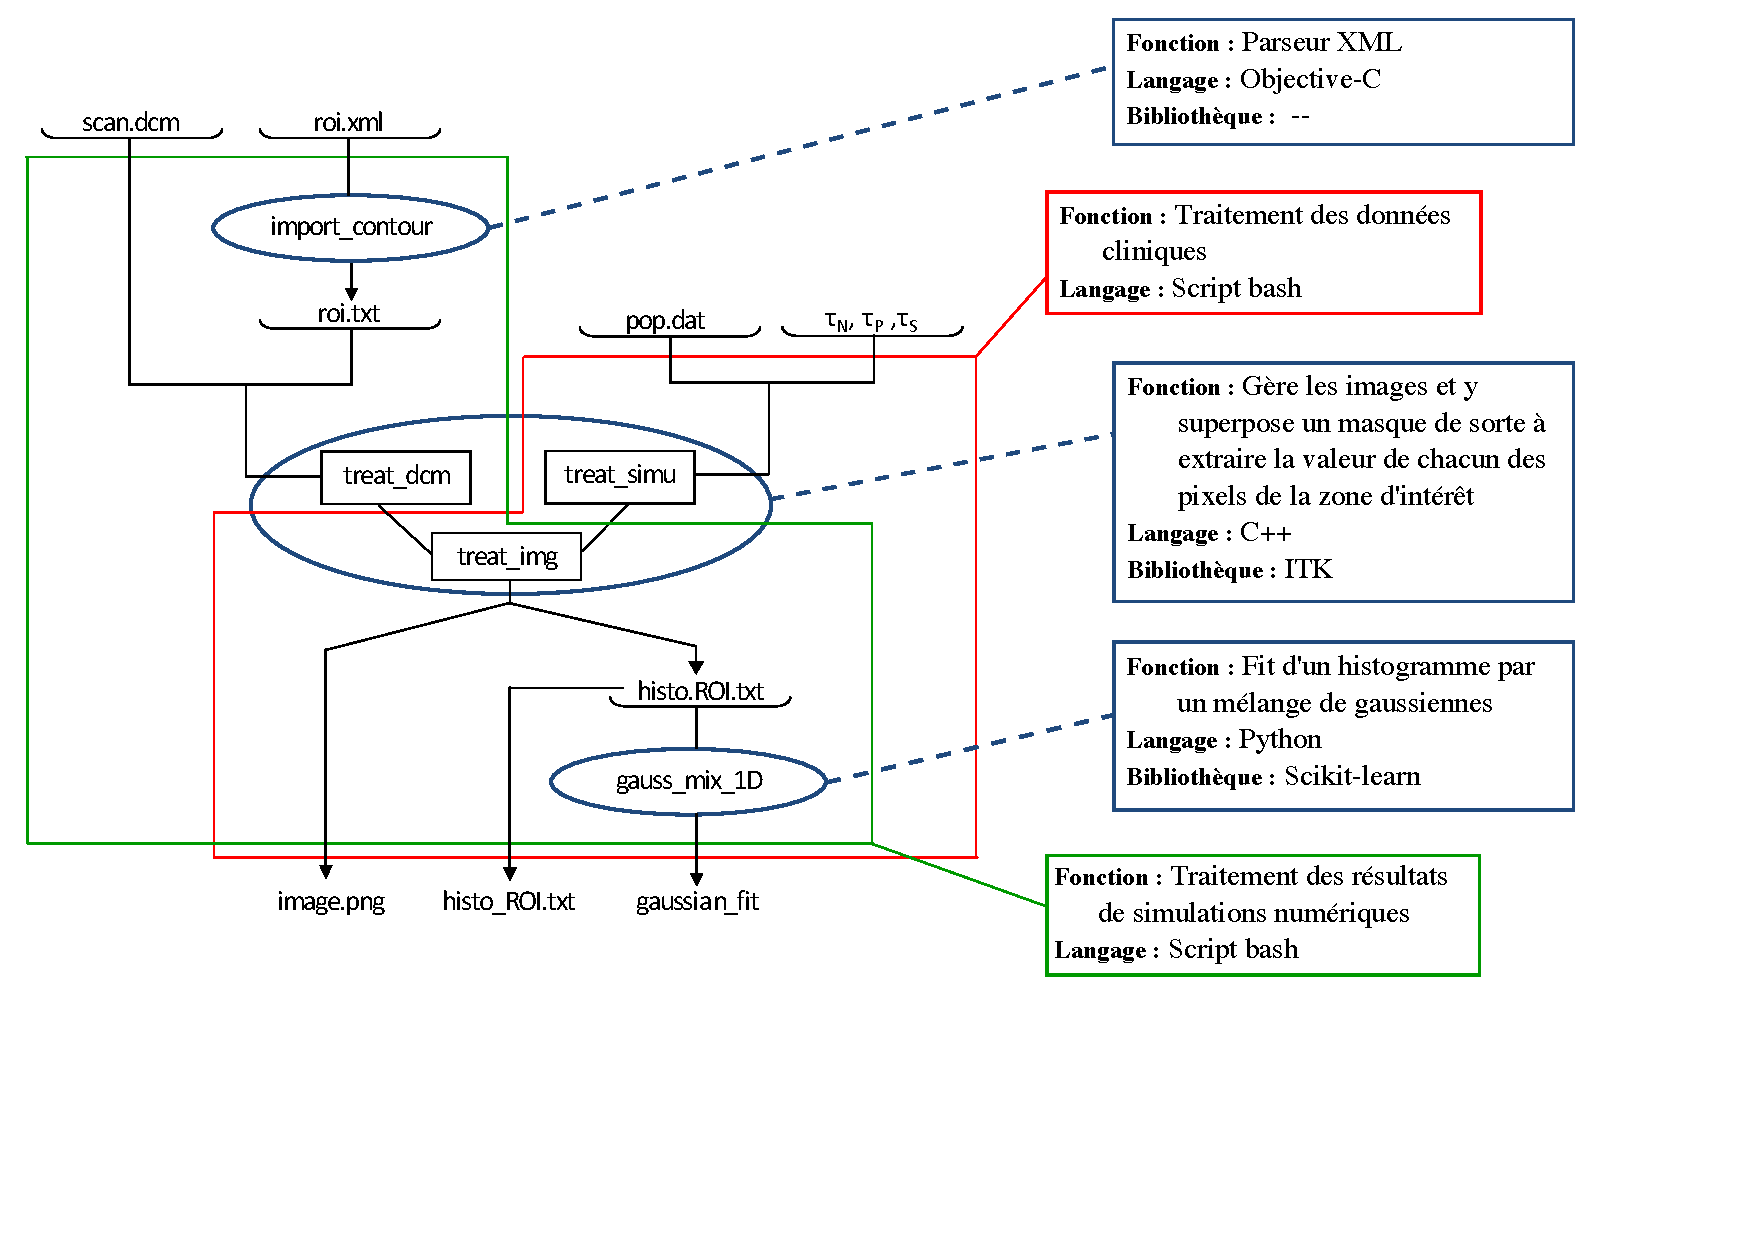
\includegraphics[width=.9\textwidth , trim = 0cm 43mm 30mm 0mm, clip=true]{schema/schema_architecture_code.pdf} %%%%  left, bottom, right and top
\caption{\label{fig:schema_struct_code}Schéma du code de calcul permettant la quantification de l'\hetero. Le code est très hétéroclite et fait intervenir plusieurs langages de programmation.}
%%\end{figure}
\end{sidewaysfigure}


\paragraph{}
Le code s'articule donc en plusieurs briques dont l'arrangement est schématisé sur la la Figure~\ref{fig:schema_struct_code}. Outre un parseur xml écrit en Objective-C, deux briques principales se distinguent. 


Une première brique a été développée en C++ avec la librairie ITK. 
Elle a pour but, à partir d'une image quelconque 
%(dicom ou sortie image fournie par le code précédent)
 et d'un contour, d'extraire les valeurs des niveaux de gris des pixels présents à l'intérieur du contour. On obtient ainsi l'histogramme des niveaux de gris. 
La librairie ITK a l'avantage de traiter des images aux formats standards (.jpg, .png, etc) mais aussi et surtout le format DICOM, qui est le format des images médicales que nous possédons. 
Puisque ce code manipule différents formats d'images, j'en ai profité pour qu'il soit capable d'exporter, depuis les données DICOM, des images dans des formats standards sur lesquelles sont mis en évidence les différents contours. 
Ce code a notamment permis de générer les images présentées dans les Figures~\ref{fig:contourageNber} et~\ref{fig:contourageChen} de l'annexe~\ref{chap:anx_img_complement} (pages~\pageref{fig:contourageNber}  et~\pageref{fig:contourageNber}).


La seconde brique est chargée de trouver les paramètres de deux gaussiennes dont la somme décrit au mieux un histogramme donné. 
Cette brique est basée sur la librairie Python Scikit-learn, qui contient un module dédié au mélange gaussien. Une fois les paramètres du mélange bi-gaussien identifiés, on peut aisément construire et examiner les critères quantifiant l'\hetero.

%L'ensemble de l'articulation entre les différents modules est présenté sur la Figure~\ref{fig:schema_struct_code}.
Afin de faciliter le chainage entre les différentes étapes du calcul, deux scripts Bash ont été développés (représenté par les cadres rouges et vert sur la Figure~\ref{fig:schema_struct_code}). Le premier permet de traiter de A à Z, les données cliniques. L'utilisateur fournit un dossier contenant un ou plusieurs scanners avec leur contourage provenant d'OsiriX. Le script fournit en sortie, des images post-traitées ainsi que les valeurs des histogrammes des niveaux de gris correspondant aux zones contourées et leur description en mélanges de gaussiennes. Le second script requiert en entrée les résultats de simulations numériques du modèle EDP, et les valeurs des 3 niveaux de gris $\tau_N, \tau_P$ et $\tau_S$. Il fournit les mêmes sorties que le premier script. 
Dans chacun de ces scripts une dernière option (non présentée sur le schéma) est disponible, pour réaliser après coup, le tracé de différents critères quantifiant l'\hetero. 
L'ensemble de la chaîne de calcul a donc été automatisée et s'exécute ainsi de manière très simple bien que sa structure interne soit hétéroclite. 


Terminons en donnant brièvement quelques statistiques. Ce deuxième code fait environ \numprint{5000} lignes. Le temps d'exécution est de quelques secondes.
 

\end{document}